\section {Vergleich reaktive \& blockierende Anwendung}
\label{section:vergleich_reaktiv_blockierend}
Um zu prüfen, ob Leistungsfähigkeit und Skalierbarkeit einer reaktiven, auf dem \newline
\verb|Multi-Reactor-Modell| und \verb|Non-blocking I/O| basierenden,
Anwendung tatsächlich die einer traditionellen, auf dem \verb|Thread per request Modell| und \verb|Blocking I/O| basierenden, Anwendung übertrifft, werden in
diesem Kapitel beide Ansätze hinsichtlich verschiedener Metriken in einem festen Zeitintervall miteinander verglichen.

Dafür werden sowohl die reaktive, als auch die nicht-reaktive Anwendung, in 5 Testreihen, jeweils zwei Lasttests unterzogen:
\begin{enumerate}
  \item Abfrage von statischen Daten
  \item Abfrage von dynamischen Daten (mit Datenbankanbindung)
\end{enumerate}
Jeder Lasttest besteht darin, clientseitig eine Reihe an Lasten (workloads) zu generieren und jede Last, über die Dauer von einer Minute,
sekündlich an einen ausgewählten HTTP-Endpunkt der Anwendung zu senden.
Dabei wird das Zeitintervall vom Starten der Anwendung bis zur Beantwortung der ersten Anfrage,
der benötigte Arbeitsspeicher und die CPU-Auslastung des Prozesses, der Durchsatz, sowie die Latenz gemessen.
Primär aus Kostengründen eignen sich für Container-, Cloud- und Serverless-Umgebungen Anwendungen die
auf schnelle Startzeiten und geringen Ressourcenverbrauch, statt auf hohen Durchsatz und lange Laufzeiten, setzen.
Aus diesem Grund werden die beiden Anwendungen den beiden Lasttests sowohl im \verb|JVM mode|, als auch im \verb|native mode|
(siehe Absatz \verb|Quarkus und native image| in Kapitel \ref{subsubsec:frameworks})
unterzogen. Insgesamt ergeben sich also 4 Testszenarien pro Anwendung.

\subsection{Implementierung \& Systemaufbau}
\label{section:implementierung}
Die beiden Anwendungen implementieren mit dem Quarkus-Framework jeweils eine simple \acrshort{rest}-Schnittstelle (\acrlong{rest})
mit HTTP-CRUD Methoden, und einer angebundenen PostgreSQL-Datenbank.
Dabei ist vor allem die HTTP-Schicht von Interesse. Die HTTP-Unterstützung von Quarkus basiert auf einem reaktiven, nicht-blockierenden
Unterbau: der \verb|Vert.x Engine| (siehe Kapitel \ref{subsubsec:reaktive_systeme}).
Jede HTTP-Anfrage wird auf einem der \verb|IO threads|
verarbeitet, und durch eine Routing-Schicht an den Anwendungscode weitergeleitet.
Abhängig vom verwendeten Ansatz zur Implementierung des jeweiligen HTTP-Endpunktes wird der Code auf unterschiedliche Art und Weise abgearbeitet.
Der Code wird entweder auf einem blockierenden \verb|Worker thread| aus dem \verb|Worker thread pool| (Servlet, \Gls{jaxrsg}(*)),
ganz nach dem \verb|Thread per request|-Modell, oder weiterhin auf einem der \verb|IO threads| (Reactive Routes, Reactive Resteasy),
nach dem \verb|Multi-Reactor-Modell|, ausgeführt.
\newpage
\begin{figure}[h]
  \centering
  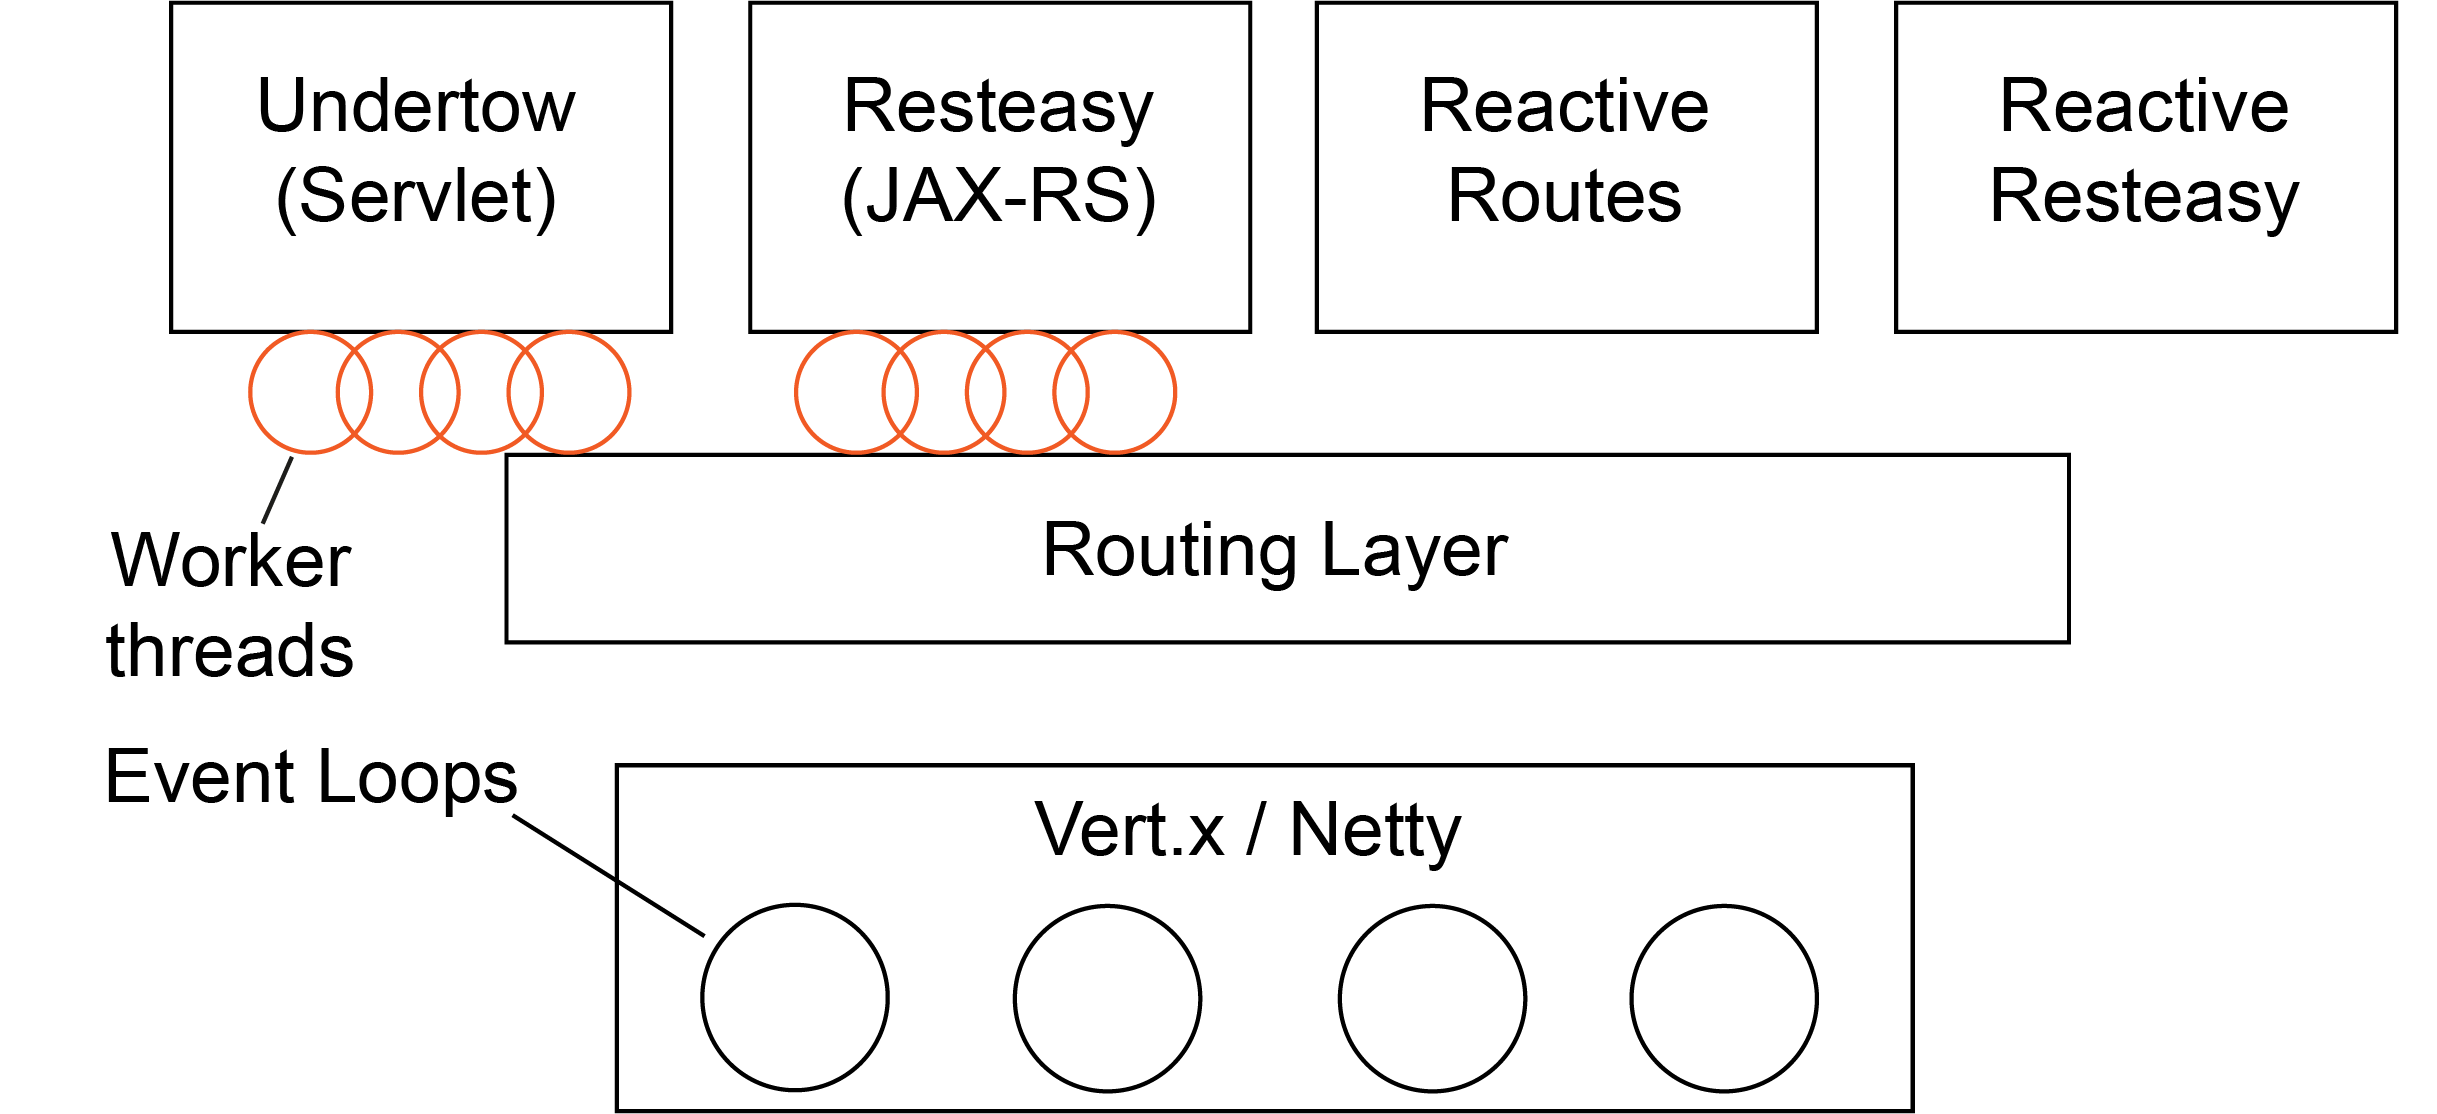
\includegraphics[width=0.9\textwidth]{Quarkus_HTTP_Layer}
  \caption{Quarkus HTTP-Schicht \parencite{QuarkusReactiveRoutes}}
  \label{fig:quarkus_http_schicht}
\end{figure}
Damit sich beide Anwendungen nahe an einer realen REST-API mit \verb|Jakarta EE| orientieren, haben
sie, zusätzlich zu den grundlegenden Abhängigkeiten des Quarkus-Frameworks, folgende Projekt-Abhängigkeiten:
\begin{itemize}
  \item \acrshort{jax-rs} Implementierung
  \item \Gls{jsong}(*) Unterstützung
  \item PostgreSQL - Datenbanktreiber
  \item \Gls{jpag}(*) Implementierung
\end{itemize}

Diese Abhängigkeiten wurden vom Quarkus Maven-Repository sowohl in blockierender,
als auch in nicht-blockierender und \verb|native image|-kompatibler Form bereitgestellt: \parencite{MavenQuarkusIO}
% space between the text and the left/right border of its containing cell is set to 18 pt
\setlength{\tabcolsep}{18pt}
% the height of each row is set to 1.5 relative to its default height
\renewcommand{\arraystretch}{1.5}
\begin{table}[ht!]
  \centering
  \begin{tabular}{| c | c | c |}
    \hline
                                  & Blockierend      & Nicht-blockierend (reaktiv) \\
    \hline
    JAX-RS                        & Resteasy         & Resteasy Reactive           \\
    \hline
    \acrshort{json}               & Resteasy-Jackson & Resteasy-Reactive-Jackson   \\
    \hline
    Datenbanktreiber              & JDBC-Postgresql  & Reactive-Pg-Client          \\
    \hline
    \acrshort{jpa}/\acrshort{orm} & Hibernate-ORM    & Hibernate-Reactive          \\
    \hline
  \end{tabular}
  \caption{Tabelle mit den Abhängigkeiten beider Applikationen}
  \label{table:dependencies}
\end{table}

In Listing \ref{lst:update_blocking} und \ref{lst:update_reactive} ist jeweils die Update Methode der REST-APIs abgebildet, um den
Unterschied der beiden Paradigmen anhand von Code darzustellen.

Dabei wird versucht eine Entity mit der übergebenen \verb|id| der HTTP-Anfrage
aus der Datenbank abzurufen und, falls eine gefunden werden konnte, dessen Name mit dem Wert
aus dem Request-Body der Anfrage zu überschreiben. Anschließend wird die Entity mit dem neuen Namen wieder in die Datenbank zurückgeschrieben
und HTTP-Statuscode 422 an den Client zurückgegeben. Falls keine Entity gefunden werden konnte, wird stattdessen
HTTP-Statuscode 404 zurückgegeben.

In der reaktiven Anwendung ist die gesamte Logik, sowie Fehler- und Nullprüfung in einer einzigen Pipeline abgebildet.
Da in diesem Beispiel Mutiny genutzt wird, wird der Rückgabetyp immer als \verb|Uni| oder \verb|Multi|-Objekt eines spezifischen Typs
angegeben. \verb|Uni| repräsentiert dabei einen Datenstrom der entweder ein Element oder ein Fehler-Event emittiert.
\verb|Multi| repräsentiert einen Datenstrom der entweder 0, 1, \verb|n| oder unendlich viele Elemente emittieren kann.
Der \verb|Subscriber| ist in diesem Fall der Aufrufer der \verb|update|-Methode und sorgt dafür, dass die Pipeline überhaupt ausgeführt wird.

Jede \verb|Pipe| der Pipeline gibt ein \verb|Uni| an den Downstream weiter.
Dieses kann entweder vom Typ \verb|Void| für null-Werte oder vom Typ der jeweiligen Entität sein.
\footnote{invoke() und call() in Listing \ref{lst:update_reactive} sind Abkürzungen, um die Lesbarkeit in Mutiny zu verbessern\parencite{MutinyShortcuts}}.

\begin{lstlisting}[caption=Update Methode der nicht-reaktiven Anwendung, language=Java, captionpos=b, label=lst:update_blocking]
  @PUT
  @Path("/{id}")
  public Response update(Fruit fruit, @PathParam("id") Long id) {
    if (fruit == null || fruit.getName() == null) {
      return Response.status(422).build();
    }
    Fruit storedFruit = fruitRepository.findById(id);
    if (storedFruit == null) {
      return Response.status(Response.Status.NOT_FOUND).build();
    }
    storedFruit.setName(fruit.getName());
    fruitRepository.update(storedFruit);
    return Response.status(Response.Status.OK).build();
  }
\end{lstlisting}

\begin{lstlisting}[caption=Update Methode der reaktiven Anwendung, language=Java, captionpos=b, label=lst:update_reactive]
@PUT
@Path("{id}")
public Uni<Response> update(Long id, Fruit fruit) {
	if (fruit == null || fruit.getName() == null) {
		return Uni.createFrom().item(Response.status(422).build());
	}
	return fruitRepository.findById(id).onItem()
	.ifNotNull().invoke(storedFruit -> storedFruit.setName(fruit.getName())
	).call(storedFruit -> fruitRepository.update(storedFruit))
			.onItem().ifNotNull().transform(storedFruit ->
			Response.ok(storedFruit).build())
			.onItem().ifNull().continueWith(Response.status(Status.NOT_FOUND).build());
}
\end{lstlisting}
Der Projekt-Code dieser Arbeit kann auf GitHub unter der URL \url{https://github.com/ErikSimonsen/Master-Thesis-Sourcecode} eingesehen und abgerufen werden.
\newpage
\subsection{Testumgebung}
\label{section:testumgebung}
Für die Testumgebung werden zwei Systeme benötigt: der Client-Host und der Server-Host.
Dabei muss es sich um UNIX-Systeme handeln, da einige der verwendeten Werkzeuge nur auf diesen Systemen verfügbar sind.
Zudem müssen beide Systeme per SSH von einem (idealerweise vorhandenem) dritten System, dem User-Host
\footnote{Dies kann allerdings auch der Client-Host selber sein}
erreichbar sein, damit dieses den Testablauf in der korrekten Abfolge ausführen kann.
Der Einfachheit halber empfiehlt es sich, dass sich alle Geräte im gleichen Netzwerk befinden.
Beide Anwendungen verwenden Version 1.12.1 des Quarkus Frameworks, welches wiederum Version 20.1 der GraalVM nutzt.
Um eine reproduzierbare Anwendungsumgebung und Ressourcenallokation zu ermöglichen, laufen beide Anwendungen auf dem Server-Host in
jeweils einem Docker-Container mit fest definierten Ressourcen:
\begin{itemize}
  \item Nutzung von 4 CPU-Kernen
  \item 1024 MB RAM
  \item 256 MB JVM-Heap Größe\footnote{Seit Java 10 wird automatisch 1/4 des Speicherlimits des Containers genutzt \parencite{Java10ReleaseNotes}}
\end{itemize}
Der Docker-Container für die PostgreSQL-Datenbank verwendet:
\begin{itemize}
  \item 4 CPU-Kerne
  \item 2048 MB RAM
\end{itemize}

Die Größe des von Vert.x verwendeten \verb|Worker thread pools| (siehe Abbildung \ref{fig:quarkus_http_schicht}) beträgt standardmäßig 20 und bleibt
unverändert. Die Größe des \verb|Event loop thread pools| hingegen wird manuell auf 8 gesetzt, da die Anwendung durch die Ressourcenallokation
des Docker-Containers nur 4 CPU-Kerne nutzen darf und jeder dieser CPU-Kerne Hyper-Threading\footnote{Wodurch jeder physische CPU-Kern über
  zwei \glsplural{logische CPU}(*) verfügt} unterstützt.
Damit kann die optimale Verteilung von einem \verb|IO thread| pro logischer CPU erreicht werden.
Standardmäßig wird die Ressourcenbegrenzung durch Container von Vert.x nicht beachtet und die Anzahl der \verb|IO threads| wird auf die doppelte
Anzahl der verfügbaren CPU-Kerne des Container-Hosts gesetzt, weswegen es der beschriebenen Anpassung bedarf.

Die Anwendung die auf dem Client-Host die \verb|workload| für die beiden zu testenden Anwendungen generiert,
nutzt in dieser Testumgebung 4 Threads.
Welche Laufzeitumgebungen und Tools für den Testaufbau auf den jeweiligen Hosts vorhanden sein müssen, und wie diese installiert werden,
wird in der README.md-Datei des Projekts beschrieben.

Da die Messergebnisse je nach verwendeter Hardware der Client- und Server-Hosts durchaus variieren können werden im Folgenden
die Systemspezifikationen der verwendeten Systeme des Authors gelistet:
\begin{table}[ht!]
  \centering
  \begin{tabular}{| c | c |}
    \hline
    Server-Host                                                  \\
    \hline
    CPU's          & AMD Ryzen 7 2700x eight-core processor x 16 \\
    \hline
    RAM            & 16 GB                                       \\
    \hline
    Speicher       & 1,5 TB                                      \\
    \hline
    Betriebssystem & Fedora 34 (Workstation Edition)             \\
    \hline
    Kernel         & Linux version \verb|5.12.14-300.fc34.x86_64|   \\
    \hline
  \end{tabular}
  \caption{Systemspezifikationen des verwendeten Server-Hosts}
  \label{table:system_host}
\end{table}

\begin{table}[ht!]
  \centering
  \begin{tabular}{| c | c |}
    \hline
    Client-Host    & Acer Aspire VN7-591G                      \\
    \hline
    CPU            & Intel® Core™ i5-4210H CPU @ 2.90GHz × 4   \\
    \hline
    RAM            & 8 GB                                      \\
    \hline
    Speicher       & 500 GB                                    \\
    \hline
    Betriebssystem & Fedora 34 (Workstation Edition)           \\
    \hline
    Kernel         & Linux version \verb|5.12.14-300.fc34.x86_64| \\
    \hline
  \end{tabular}
  \caption{Systemspezifikationen des verwendeten Client-Hosts}
  \label{table:system_client}
\end{table}

\subsection{Testaufbau}
\label{section:testaufbau}
Der im Folgenden erläuterte Testaufbau basiert auf einer, vom Autor erweiterten, Architektur die vom Quarkus-Entwicklerteam
zur Erstellung von verschiedenen Benchmarks für den Quarkus Technologie-Stack genutzt wurde.
\parencite{QuarkusBlog, QuarkusJohnaohara}

Um den gesamten Testablauf zu automatisieren, und über mehrere Hosts zu steuern wird ein Tool namens qDup eingesetzt.
Damit können Shell-Kommandos als Skripte gruppiert, und verschiedenen Hosts je nach Rolle zugewiesen werden.
\footnote{Die qDup Skripte mit dem gesamten Testablauf können im Verzeichnis \textit{/scripts/qDup} des Quellcodeverzeichnisses eingesehen und
  angepasst werden.}

Um dem Ablauf korrekt zu steuern werden Signale definiert die ein Host sendet, und auf welche die anderen Hosts warten, um ihrerseits
weitere Skripte auszuführen.
\footnote{Beispielsweise sollte der Server-Host erst anfangen den Java-Prozess zu überwachen, sobald der Client-Host die \textit{workload}
  generiert und nicht bereits davor}

Wie bereits in Kapitel \ref{section:testumgebung} angedeutet, nutzt qDup SSH um auf die jeweilige Hosts zuzugreifen.
Im ersten Schritt \textit{build applications} wird auf dem Server-Host das Quellcodeverzeichnis geklont und beide Anwendungen werden
jeweils als \gls{uber-jar}(*), für ein einfaches Deployment in den Docker-Container, und als \verb|native image| gebaut.

Anschließend wird über ein JavaScript-Skript, welches in der Laufzeitumgebung Node.js läuft,
die \verb|Mean Start Time to First Request|, also das durchschnittliche Zeitintervall zwischen dem Start einer Anwendung bis
zur Verarbeitung der ersten Anfrage gemessen.
Dabei wird die Anwendung ohne Docker-Container auf dem Server-Host ausgeführt und die Zeitmessung gestartet. Anschließend werden in einer Schleife
solange HTTP-Anfragen an einen Endpunkt der Anwendung geschickt bis der HTTP-Statuscode 200 zurückgeliefert wird, was das Ende der Messung markiert.
Dieser Prozess wird mehrfach durchgeführt und die gemessenen Zeiten in einer Textdatei gespeichert.
Aus diesen Werten wird in der Auswertung der Daten dann der Durchschnitt gebildet.
Darüber hinaus werden in diesem Schritt die Docker-Container der Datenbank
\footnote{Nur beim Test mit dynamischen Daten} und der beiden REST-APIs gebaut.\newline

Beim zweiten Schritt \textit{run applications} wird der Docker-Container der jeweiligen Anwendung gestartet und anschließend signalisiert,
dass die Anwendung nun bereit ist.
Daraufhin wird auf dem Client-Host das Skript \textit{generate load} gestartet.
Die \verb|workload| ist hier definiert als die Anzahl der an den Server-Host versendeten HTTP-Anfragen \textit{pro Sekunde}.
Für das Generieren und Übermitteln der \verb|workload| wird das Werkzeug \verb|wrk2| genutzt, welches das
bewährte HTTP-Benchmarking Tool \verb|wrk| um folgende Funktionen erweitert:\parencite{Wrk2, Wrk}
\begin{enumerate}
  \item Definierbarer konstanter Durchsatz (workload)
  \item Korrektere Messung der Antwort-Latenz durch\newline Vermeidung von \verb|Coordinated Omission|
  \item Hochexaktes Messen durch \Glsuseri{hdrHistogramm}(*)
\end{enumerate}

\paragraph{Coordinated Omission Problem}
Der Begriff \verb|Coordinated Omission Problem| wurde von Gil Tene, CTO und Mitgründer von Azul Systems, um 2012 geprägt.
Koordinierte Auslassung beschreibt in diesem Kontext das Problem, dass sich ein Messsystem unabsichtlich so mit dem zu messenden System   koordiniert,
dass es vermieden wird Ausreißer zu messen.

Viele Lastgeneratoren berechnen die Latenz für eine Anfrage als die vergangene Zeit zwischen dem Senden des ersten Bytes einer Anfrage
bis zum Erhalt der kompletten Antwort. Während dieses Modell die tatsächliche Bearbeitungszeit individueller Anfragen korrekt misst,
liegt dabei ein starker koordinierter Auslassungseffekt vor,
wodurch die meisten Artefakte mit hoher Latenz, die der gemessene Server aufweist, ignoriert werden.
Da jede Verbindung erst anfängt eine neue Anfrage zu senden nachdem eine Antwort bezüglich der vorherigen Anfrage erhalten wurde,
resultieren Antworten mit hoher Latenz darin, dass der Lastgenerator in einem bestimmten Zeitintervall weniger Anfragen an den Server schickt als in einer
Phase niedriger Latenz, da die nachfolgenden Anfragen verzögert werden. Ähnlich wie bei \verb|Event Loops| \textit{blockieren}
Anfragen mit hoher Latenz also das Absenden weiterer Anfragen.

Folglich ist die clientseitig generierte Arbeitslast in Phasen hoher serverseitiger Latenz deutlich geringer als in Phasen niedriger Latenz, da
sie von der Antwortzeit des Servers beeinflusst wird. Die vom Server zu bearbeitende Last ist also nicht konstant.\parencite{mci/Friedrich2017}
\newpage
\verb|Wrk2|, dessen Author auch Gil Tene ist, umgeht das \verb|Coordinated Omission Problem| in dem es eine konstante Lasterzeugung (als Befehlsargument) mit
einer Latenzmessung, die den beabsichtigten ebenso konstanten Durchsatz berücksichtigt, kombiniert.

Dabei wird die Antwortlatenz nicht ab dem Zeitpunkt gemessen, zu dem die tatsächliche Übertragung einer Anfrage aufgetreten ist.
Stattdessen misst wrk2 die Antwortlatenz ab dem Zeitpunkt zu dem die Übertragung,
gemäß dem konstanten Durchsatz, hätte erfolgen \textit{sollen} bis zum Erhalt der vollständigen Antwort.\parencite{Wrk2}\newline

Pro Test (siehe Anfang Kapitel \ref{section:vergleich_reaktiv_blockierend}) werden Benchmarks für eine ganze Reihe an \verb|workloads| gemessen.
Jede \verb|workload| wird sekündlich über einen Zeitraum von 60 Sekunden über 100 offene HTTP-Verbindungen an den Server-Host übermittelt.
In den Tests nutzt \verb|wrk2| 4 Threads für das Generieren und Übermitteln der \verb|workloads|, sowie das Messen der Antwortzeit.

Damit der Anwendungscode des angesteuerten HTTP-Endpunkts durch den JIT-Compiler (siehe Absatz \verb|Quarkus und native image| in Kapitel
\ref{subsubsec:frameworks}) optimiert wird, findet pro \verb|workload| vor der eigentlichen Mess-Phase eine identische Warmup-Phase statt.

Listing \ref*{lst:generateLoad} zeigt den Aufruf von \verb|wrk2| mit den beschriebenen Parametern in der Warmup- und Mess-Phase.
\verb|${{RUN_RATE}}| enthält dabei die momentane \verb|workload|, \verb|${{RUNTIME.name}}| den Namen der Anwendung und \verb|${{TEST_DYNAMIC_ENDPOINT}}| den
URI des API-Endpunktes mit dynamischen Daten.
\footnote{Das Ausführen der Makefile des wrk2-Projektes produziert ein executable namens wrk statt wrk2}

\begin{lstlisting}[caption=Auszug des qDup Skripts generate load, captionpos=b, label=lst:generateLoad]
- signal: ${{RUNTIME.name}}-${{RUN_RATE}}-WARM-UP-START
- sh: wrk -t 4 -c 100 -d 60s -R ${{RUN_RATE}} ${{TEST_DYNAMIC_ENDPOINT}} > ${{CLIENT_FILE_PATH}}/output/${{RUNTIME.name}}-${{RUN_RATE}}-WARM-UP.wrk2.out
- signal: ${{RUNTIME.name}}-${{RUN_RATE}}-WARM-UP-END
- sh: sleep 5s
- signal: ${{RUNTIME.name}}-${{RUN_RATE}}-MEASURE-START
- sh: wrk -t 4 -c 100 -d 60s -R ${{RUN_RATE}} --latency ${{TEST_DYNAMIC_ENDPOINT}} > ${{CLIENT_FILE_PATH}}/output/${{RUNTIME.name}}-${{RUN_RATE}}-MEASURE.wrk2.out
- signal: ${{RUNTIME.name}}-${{RUN_RATE}}-MEASURE-END
   \end{lstlisting}

Die Ausgabe von wrk2 enthält Informationen zur \Gls{latenz}\footnote{Pro verwendetem Thread und Gesamt},
zum \Gls{durchsatz} und der \Gls{perzentile}(*) der \Gls{latenz}, welche durch ein \acrshort{hdrhistogram} dargestellt wird.
Listing \ref*{lst:wrk-listing} zeigt die umgeleitete Ausgabe ohne die genaue Darstellung der Perzentile.

\begin{lstlisting}[caption=Beispiel für Ausgabe von wrk,captionpos=b, label=lst:wrk-listing]
Running 1m test @ http://erik-pc.local:8080/greeting/Bob
4 threads and 100 connections
Thread calibration: mean lat.: 310.434ms, rate sampling interval: 1047ms
Thread calibration: mean lat.: 330.365ms, rate sampling interval: 1127ms
Thread calibration: mean lat.: 298.671ms, rate sampling interval: 994ms
Thread calibration: mean lat.: 333.465ms, rate sampling interval: 1123ms
Thread Stats   Avg      Stdev     Max   +/- Stdev
	Latency     1.76s   738.93ms   4.12s    62.98%
	Req/Sec    28.58k   633.82    30.09k    66.49%
6839722 requests in 1.00m, 476.17MB read
Requests/sec: 113929.77
Transfer/sec:      7.93MB
\end{lstlisting}

Bevor die Warmup- und die Belastungs-Phase vom Client-Host ausgeführt werden, wird dem Server-Host signalisiert, dass
er das Skript \textit{capture platform stats} ausführen soll.
In diesem Skript wird, wie in Listing \ref{lst:top-listing} gezeigt, die Observation des Anwendungs-Prozesses durch das Kommandozeilenprogramm \verb|top| gestartet.
\verb|Top| wird dabei im Batch-Modus gestartet mit einer Wiederholrate von einer Sekunde.
Die Prozess-Zeile der Ausgabe von \verb|top| enthält eine Vielzahl an Informationen zu dem beobachteten Prozess.\parencite{linuxTopManual}

Von besonderem Interesse sind hierbei die CPU-Auslastung und der verwendete Arbeitsspeicher des Prozesses.

\begin{lstlisting}[language=sh, caption=Auszug des qDup Skripts capture-platform-stats, captionpos=b, label=lst:top-listing]
- wait-for: ${{RUNTIME.name}}-${{RUN_RATE}}-WARM-UP-START
- sh: top -b  -d 1 -p ${{RUN.JAVA_APP_PID}} | grep java > ${{SERVER_FILE_PATH}}/output/${{RUNTIME.name}}-${{RUN_RATE}}-WARM-UP-top.out &
- sh: export TOP_PID=$!
- wait-for: ${{RUNTIME.name}}-${{RUN_RATE}}-WARM-UP-END
- sh: kill -9 $TOP_PID
- wait-for: ${{RUNTIME.name}}-${{RUN_RATE}}-MEASURE-START
- sh: top -b  -d 1 -p ${{RUN.JAVA_APP_PID}} | grep java > ${{SERVER_FILE_PATH}}/output/${{RUNTIME.name}}-${{RUN_RATE}}-MEASURE-top.out &
- sh: export TOP_PID=$!
- wait-for: ${{RUNTIME.name}}-${{RUN_RATE}}-MEASURE-END
- sh: kill -9 $TOP_PID
\end{lstlisting}

Im letzten Schritt werden die Ausgaben von \verb|wrk2| und \verb|top| über SSH vom Client- und Server-Host auf den User-Host,
der das qDup Skript ausgeführt hat, kopiert.
In Abbildung \ref{fig:testaufbau} wird der beschriebene Testaufbau und dessen Durchführung dargestellt.
\begin{figure}[ht]
  \centering
  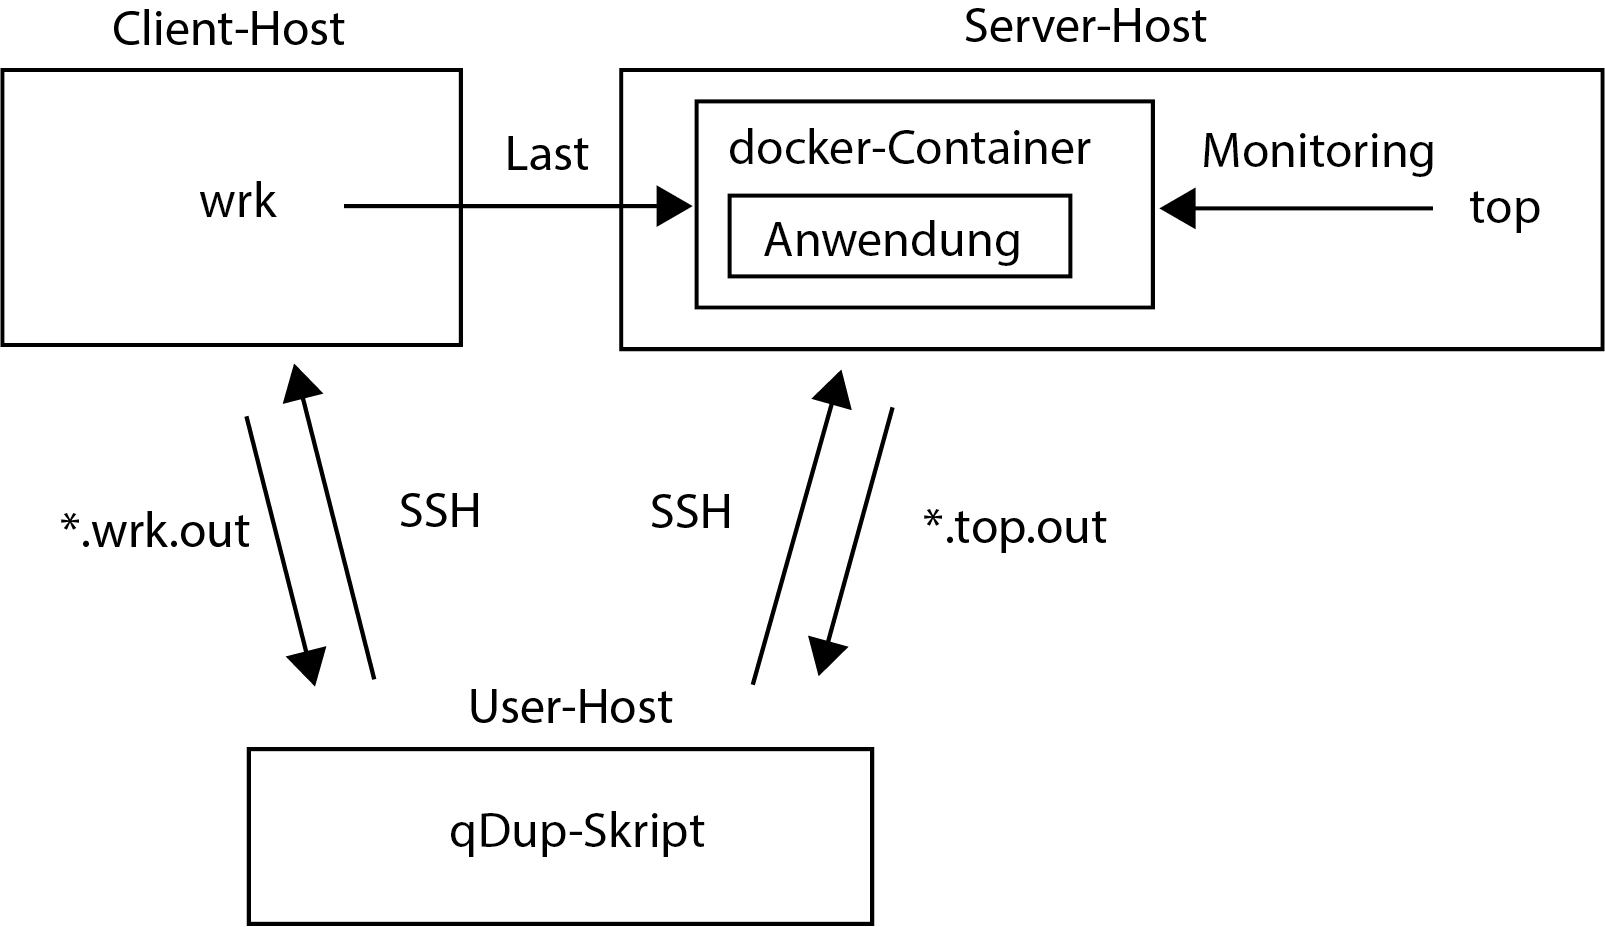
\includegraphics[width=0.7\textwidth]{Testaufbau}
  \caption{Testaufbau}
  \label{fig:testaufbau}
\end{figure}

Die Ausgaben von \verb|top| und \verb|wrk| werden anschließend für jede einzelne \verb|workload| eines Lasttests durch ein Java-Skript, welches mit
dem Tool \textit{JBang}\footnote{JBang erlaubt das direkte Ausführen von .java Dateien auf einer Shell} ausgeführt wird, eingelesen, geparsed und ausgewertet.
Dabei wird jeweils der Durchschnitt, das Minimum und das Maximum von Durchsatz und dazugehöriger Latenz, Speicherverbrauch und CPU-Auslastung pro Last ermittelt.
Die Resultate werden dann für die visuelle Darstellung in eine \verb|.json|-Datei geschrieben.
Abschließend werden die aufbereiteten Daten durch die Node.js-Bibliothek \textit{d3node-linechart} als Liniendiagramme visuell dargestellt.

\subsection{Test: Statische Daten}
\label{subsection:statische_daten}
Im Folgenden werden die Testresultate der \verb|2.| Testreihe dargestellt, erläutert und anschließend zusammengefasst.
Die Ergebnisse der anderen Testreihen liegen in den gleichen Größenordnungen und können im Projektverzeichnis unter \verb|results/data| und \verb|results/graphs| eingesehen werden.
Der Lasttest mit statischen Daten wird ohne Datenbankanbindung durchgeführt und der angesteuerte Endpunkt \verb|/greeting/{name}| gibt bei beiden Anwendungen
jeweils einen statischen String zurück. Wie bereits zu Beginn des Kapitels erwähnt, wird jede Anwendung sowohl im \verb|JVM mode| als auch im
\verb|native mode| getestet.
Die qDup-Skripte befinden sich im Projektverzeichnis im Verzeichnis \verb|scripts/benchmark-jvm-static.yaml| und
\verb|scripts/benchmark-native-static.yaml|.

\subsubsection{JVM mode}
\label{subsubsec:static_jvm_mode}
Wie aus Listing \ref{lst:starttimes_jvm_static} berechnet werden kann, liegt die \verb|Mean Start Time to First Request|
ohne Datenbankanbindung bei einer reaktiven Anwendung im \verb|JVM mode| bei 1353 ms und bei einer
blockierenden Anwendung bei 1516,6 ms.
\begin{lstlisting}[caption=Startzeiten im JVM mode mit statischen Ressourcen, captionpos=b, label=lst:starttimes_jvm_static]
    1356 ms     1531 ms
    1337 ms     1504 ms
    1315 ms     1495 ms
    1349 ms     1509 ms
    1408 ms     1544 ms
\end{lstlisting}

In Abbildung \ref{fig:jvm_static_mean_response} wird die durchschnittlich Latenz für den gemessenen Durchsatz jeder \verb|workload| dargestellt.
Die höchste getestete \verb|workload| beträgt bei der reaktiven Anwendung \textbf{142.000} Anfragen/Sekunde und bei der
nicht-reaktiven Anwendung \textbf{71.000} Anfragen/Sekunde.

Der maximale serverseitige Durchsatz der nicht-reaktiven Anwendung beträgt \textbf{69.000} Anfragen/Sekunde mit einer
Latenz von 217,5 ms und
die reaktive Anwendung erreicht \textbf{140.000} Anfragen/Sekunde bei einer durchschnittlichen Latenz von 646,5 ms.
Bei höheren Lasten steigt die durchschnittliche Latenz auf deutlich über eine Sekunde, weswegen der Durchsatz stagniert.

Die reaktive Anwendung erreicht also in der vorliegenden Testumgebung, für einen trivialen
Endpunkt mit statischen Daten, mehr als den doppelten Durchsatz.
\newpage
\begin{figure}[ht!]
  \includegraphics[width=1.0\textwidth]{run2/jvm-static/mean-response-vs-throughput}
  \caption{Test im JVM mode mit statischen Ressourcen: Durchschnittliche Latenz}
  \label{fig:jvm_static_mean_response}
\end{figure}
Abbildung \ref{fig:jvm_static_mean_rss} stellt den durchschnittlich allokierten Speicher des jeweiligen Anwendungsprozesses
für jede \verb|workload| dar. Der allokierte Speicher für die genannten maximalen Durchsätze beträgt dabei bei
der reaktiven Anwendung \verb|580 MB| und bei der blockierenden, nicht-reaktiven Anwendung \verb|843 MB|.
\newpage
\begin{figure}[ht!]
  \includegraphics[width=1.0\textwidth]{run2/jvm-static/mean-rss-vs-throughput}
  \caption{Test im JVM mode mit statischen Ressourcen:: Allokierter Hauptspeicher}
  \label{fig:jvm_static_mean_rss}
\end{figure}
In Abbildung \ref{fig:jvm_static_avg_cpu} wird abschließend die durchschnittlich gemessene CPU-Auslastung für jede \verb|workload|
dargestellt. Bei der nicht-reaktiven Anwendung wird eine Auslastung von 100\% bereits bei einer Last von
50.000 Anfragen/Sekunde erreicht. Die reaktive Anwendung hingegen erreicht diese Auslastung erst bei 110.000 Anfragen/Sekunde.
\newpage
\begin{figure}[ht!]
  \centering
  \includegraphics[width=1.0\textwidth]{run2/jvm-static/average-cpu-vs-throughput}
  \caption{Test mit statischen Ressourcen im JVM mode: CPU Auslastung pro workload}
  \label{fig:jvm_static_avg_cpu}
\end{figure}

In Tabelle \ref{table:static_jvm_measurement_results} werden die Resultate der gemessenen Benchmarks zusammengefasst
und zueinander ins Verhältnis gesetzt.
Im \verb|JVM mode| mit statischen Ressourcen weist die reaktive Anwendung eine 10,8\% schnellere \verb|Mean Start Time to First Request|
sowie einen 31,2\% geringeren Speicherverbrauch auf.
Darüber hinaus wird ein um etwa 102\% höherer maximaler Durchsatz erzielt, bevor die Latenz einen Wert von einer Sekunde übersteigt.
Außerdem können 120\% mehr Anfragen pro Sekunde verarbeitet werden bis die durchschnittliche CPU-Auslastung, mit dem in Tabelle
\ref{table:system_host} genannten CPU, bei 4 Kernen 100\% erreicht.

\begin{table}[ht!]
  \begin{tabular}{|l | c | c | c|}
    \hline
    Run 2 - JVM mode - static & Blockierend & Reaktiv & Verhältnis \\
    \hline
    \makecell[l]{Mean Start Time to                                \\ First Request (ms)} & 1516,6      & 1353  & 89,2\%     \\
    \hline
    Max. allokierter RAM (MB) & 843         & 580     & 68,8\%     \\
    \hline
    Max. Durchsatz (req/sec)  & 69.000      & 140.000 & 202\%      \\
    \hline
    \makecell[l]{CPU Auslastung bei 100\%                          \\ (req/sec)} & 50.000 & 110.000 & 220\%  \\
    \hline
  \end{tabular}
  \caption{Verhältnis der Benchmarks im JVM mode mit statischen Ressourcen}
  \label{table:static_jvm_measurement_results}
\end{table}

\subsubsection{native mode}
\label{subsubsec:static_native_mode}
Wie aus Listing \ref{lst:starttimes_native_static} berechnet werden kann, liegt die \verb|Mean Start Time to First Request|
ohne Datenbankanbindung, sowohl bei einer reaktiven Anwendung als auch bei einer blockierenden
Anwendung im \verb|native mode|, bei 27,6 ms.
\begin{lstlisting}[caption=Startzeiten im native mode mit statischen Ressourcen, captionpos=b, label=lst:starttimes_native_static]
    27 ms     27 ms
    27 ms     27 ms
    28 ms     29 ms
    29 ms     27 ms
    27 ms     28 ms
\end{lstlisting}

In Abbildung \ref{fig:native_static_mean_response} wird die durchschnittlich Latenz für den gemessenen Durchsatz jeder \verb|workload| dargestellt.
Die höchste getestete \verb|workload| beträgt bei der reaktiven Anwendung \textbf{76.000} Anfragen/Sekunde und bei der
nicht-reaktiven Anwendung \textbf{39.000} Anfragen/Sekunde.

Der maximale serverseitige Durchsatz der nicht-reaktiven Anwendung beträgt \textbf{37.000} Anfragen/Sekunde mit einer
Latenz von 283,3 ms und
die reaktive Anwendung erreicht \textbf{74.000} Anfragen/Sekunde bei einer durchschnittlichen Latenz von 680,6 ms.
Bei höheren Lasten steigt die Latenz auf deutlich über eine Sekunde, weswegen der Durchsatz stagniert.

\begin{figure}[ht!]
  \centering
  \includegraphics[width=1.0\textwidth]{run2/native-static/mean-response-vs-throughput}
  \caption{Test im native mode mit statischen Ressourcen: Durchschnittliche Latenz}
  \label{fig:native_static_mean_response}
\end{figure}
\newpage
Abbildung \ref{fig:native_static_mean_rss} stellt den durchschnittlich allokierten Speicher des jeweiligen Anwendungsprozesses
im Hauptspeicher für jede \verb|workload| dar. Der allokierte Speicher für die genannten maximalen Durchsätze beträgt dabei bei
der reaktiven Anwendung \verb|364 MB| und bei der blockierenden, nicht-reaktiven Anwendung \verb|564 MB|.
\begin{figure}[ht!]
  \centering
  \includegraphics[width=1.0\textwidth]{run2/native-static/mean-rss-vs-throughput}
  \caption{Test im native mode mit statischen Ressourcen: Allokierter Hauptspeicher}
  \label{fig:native_static_mean_rss}
\end{figure}

In Abbildung \ref{fig:native_static_avg_cpu} wird abschließend die durchschnittlich gemessene CPU-Auslastung für jede \verb|workload|
dargestellt. Bei der nicht-reaktiven Anwendung wird eine Auslastung von 100\% bereits bei einer Last von
34.000 Anfragen/Sekunde erreicht. Die reaktive Anwendung hingegen erreicht diese Auslastung erst bei 50.000 Anfragen/Sekunde.
\newpage
\begin{figure}[ht!]
  \centering
  \includegraphics[width=1.0\textwidth]{run2/native-static/average-cpu-vs-throughput}
  \caption{Test im native mode mit statischen Ressourcen: CPU Auslastung}
  \label{fig:native_static_avg_cpu}
\end{figure}

In Tabelle \ref{table:static_native_measurement_results} werden die Resultate der gemessenen Benchmarks zusammengefasst
und zueinander ins Verhältnis gesetzt. Im JVM mode mit statischen Ressourcen weist die reaktive Anwendung
die gleiche \verb|Mean Start Time to First Request|, sowie
einen um 35,5\% geringeren Speicherverbrauch auf.
Darüber hinaus wird ein 100\% höherer maximaler Durchsatz erzielt, bevor die Latenz eine Sekunde übersteigt.
Außerdem können 66,6\% mehr Anfragen pro Sekunde verarbeitet werden bis die durchschnittliche CPU-Auslastung 100\% erreicht.

\begin{table}[ht!]
  \begin{tabular}{|l | c | c | c|}
    \hline
    Run 2 - native mode - static & Blockierend & Reaktiv & Verhältnis \\
    \hline
    \makecell[l]{Mean Start Time to                                   \\ First Request (ms)} &   27,6    &  27,6  &   100\%   \\
    \hline
    Max. allokierter RAM (MB)    & 564         & 364     & 64,5\%     \\
    \hline
    Max. Durchsatz (req/sec)     & 37.000      & 74.000  & 200\%      \\
    \hline
    \makecell[l]{CPU Auslastung bei 100\%                             \\ (req/sec)} & 30.000 & 50.000 & 166,6\%  \\
    \hline
  \end{tabular}
  \caption{Verhältnis der Benchmarks im native mode mit statischen Ressourcen}
  \label{table:static_native_measurement_results}
\end{table}
\newpage
\subsection{Test: Datenbankzugriffe}
\label{section:datenbankzugriffe}
Im Folgenden werden die Testresultate der \verb|5.| Testreihe dargestellt und erläutert.
Die Ergebnisse der anderen Testreihen liegen in den gleichen Größenordnungen und können im Projektverzeichnis unter \verb|results/data| und \verb|results/graphs| eingesehen werden.
Der Lasttest mit dynamischen Daten wird mit Datenbankanbindung durchgeführt und der angesteuerte Endpunkt \verb|/fruits| gibt bei beiden Anwendungen
jeweils alle Elemente der Tabelle \textit{fruits} zurück. Wie bereits zu Beginn des Kapitels erwähnt, wird jede Anwendung sowohl im \verb|JVM mode| als auch im
\verb|native mode| getestet, die qDup-Skripte befinden sich im Projektverzeichnis im Verzeichnis \verb|scripts/benchmark-jvm-db.yaml| und
\verb|scripts/benchmark-native-db.yaml|.

\subsubsection{JVM mode}
\label{subsubsec:dynamic_jvm_mode}
Wie aus Listing \ref{lst:starttimes_jvm_dynamic} berechnet werden kann, liegt die \verb|Mean Start Time to First Request|
mit Datenbankanbindung bei einer reaktiven Anwendung im \verb|JVM mode| bei 1349 ms und bei einer
blockierenden Anwendung bei 1631,2 ms.

\begin{lstlisting}[caption=Startzeiten im native mode mit dynamischen Ressourcen, captionpos=b, label=lst:starttimes_jvm_dynamic]
    1345 ms    1674 ms
    1366 ms    1617 ms
    1364 ms    1656 ms 
    1324 ms    1619 ms 
    1346 ms    1590 ms 
\end{lstlisting}
In Abbildung \ref{fig:jvm_dynamic_mean_response} wird die durchschnittlich Latenz für den gemessenen Durchsatz jeder \verb|workload| dargestellt.
Die höchste getestete \verb|workload| beträgt bei der reaktiven Anwendung \textbf{37.000} Anfragen/Sekunde und bei der
nicht-reaktiven Anwendung \textbf{28.000} Anfragen/Sekunde.

Der maximale serverseitige Durchsatz der nicht-reaktiven Anwendung beträgt \textbf{26.000} Anfragen/Sekunde mit einer
Latenz von 56,6 ms und
die reaktive Anwendung erreicht \textbf{36.000} Anfragen/Sekunde bei einer durchschnittlichen Latenz von 253,8 ms.
Bei höheren Lasten steigt die Latenz auf deutlich über eine Sekunde, weswegen der Durchsatz stagniert.
\newpage
\begin{figure}[ht!]
  \centering
  \includegraphics[width=1.0\textwidth]{run5/jvm-db/mean-response-vs-throughput}
  \caption{Test im JVM mode mit dynamischen Daten: Durchschnittliche Latenz}
  \label{fig:jvm_dynamic_mean_response}
\end{figure}
Abbildung \ref{fig:jvm_dynamic_mean_rss} stellt den durchschnittlich allokierten Speicher des jeweiligen Anwendungsprozesses
im Hauptspeicher für jede \verb|workload| dar. Der allokierte Speicher für die genannten maximalen Durchsätze beträgt dabei bei
der reaktiven Anwendung \verb|573 MB| und bei der blockierenden, nicht-reaktiven Anwendung \verb|754 MB|.
\newpage
\begin{figure}[ht!]
  \centering
  \includegraphics[width=1.0\textwidth]{run5/jvm-db/mean-rss-vs-throughput}
  \caption{Test im JVM mode mit dynamischen Ressourcen: Allokierter Hauptspeicher}
  \label{fig:jvm_dynamic_mean_rss}
\end{figure}

In Abbildung \ref{fig:jvm_dynamic_avg_cpu} wird abschließend die durchschnittlich gemessene CPU-Auslastung für jede \verb|workload|
dargestellt. Bei der nicht-reaktiven Anwendung wird eine Auslastung von 100\% bereits bei einer Last von
20.000 Anfragen/Sekunde erreicht. Die reaktive Anwendung hingegen erreicht diese Auslastung erst bei 36.000 Anfragen/Sekunde.
\newpage
\begin{figure}[ht!]
  \centering
  \includegraphics[width=1.0\textwidth]{run5/jvm-db/average-cpu-vs-throughput}
  \caption{Test im JVM mode mit dynamischen Ressourcen: CPU Auslastung}
  \label{fig:jvm_dynamic_avg_cpu}
\end{figure}

In Tabelle \ref{table:dynamic_jvm_measurement_results} werden die Resultate der gemessenen Benchmarks zusammengefasst
und zueinander ins Verhältnis gesetzt.
Im JVM mode mit dynamischen Ressourcen weist die reaktive Anwendung
eine 17,4\% schnellere \verb|Mean Start Time to First Request| sowie einen um 24,1\% geringeren Speicherverbrauch auf.
Darüber hinaus wird ein um etwa 38\% höherer maximaler Durchsatz erzielt, bevor die Latenz eine Sekunde übersteigt.
Außerdem können 80\% mehr Anfragen pro Sekunde verarbeitet werden bis die CPU Auslastung 100\% erreicht.

\begin{table}[ht!]
  \begin{tabular}{|l | c | c | c|}
    \hline
    Run 5 - JVM mode - dynamic & Blockierend & Reaktiv & Verhältnis \\
    \hline
    \makecell[l]{Mean Start Time to                                 \\ First Request (ms)} &   1631,2    &  1349  &   82,6\%   \\
    \hline
    Max. allokierter RAM (MB)  & 754         & 573     & 75,9\%     \\
    \hline
    Max. Durchsatz (req/sec)   & 26.000      & 36.000  & 138\%      \\
    \hline
    \makecell[l]{CPU Auslastung bei 100\%                           \\ (req/sec)} & 20.000 & 36.000 & 180\%  \\
    \hline
  \end{tabular}
  \caption{Verhältnis der Benchmarks im JVM mode mit dynamischen Ressourcen}
  \label{table:dynamic_jvm_measurement_results}
\end{table}

\newpage
\subsubsection{native mode}
\label{subsubsec:dynamic_native_mode}
Wie aus Listing \ref{lst:starttimes_native_dynamic} berechnet werden kann, liegt die \verb|Mean Start Time to First Request|
mit Datenbankanbindung bei einer reaktiven Anwendung im \verb|native mode| bei 27,8 ms und bei
einer blockierenden Anwendung bei 46 ms.

\begin{lstlisting}[caption=Startzeiten im JVM mode mit dynamischen Ressourcen, captionpos=b, label=lst:starttimes_native_dynamic]
    27 ms   56 ms
    28 ms   45 ms
    28 ms   46 ms
    27 ms   37 ms
    29 ms   46 ms
\end{lstlisting}

In Abbildung \ref{fig:native_dynamic_mean_response} wird die durchschnittlich Latenz für den gemessenen Durchsatz jeder \verb|workload| dargestellt.
Die höchste getestete \verb|workload| beträgt bei der reaktiven Anwendung \textbf{20.000} Anfragen/Sekunde und bei der
nicht-reaktiven Anwendung \textbf{16.000} Anfragen/Sekunde.

Der maximale serverseitige Durchsatz der nicht-reaktiven Anwendung beträgt \textbf{15.500} Anfragen/Sekunde mit einer
Latenz von 80,5 ms und
die reaktive Anwendung erreicht \textbf{18.500} Anfragen/Sekunde bei einer durchschnittlichen Latenz von 14,3 ms.
Bei höheren Lasten steigt die Latenz auf deutlich über eine Sekunde, weswegen der Durchsatz stagniert.

\begin{figure}[ht!]
  \centering
  \includegraphics[width=1.0\textwidth]{run5/native-db/mean-response-vs-throughput}
  \caption{Test im native mode mit dynamischen Ressourcen: Durchschnittliche Latenz}
  \label{fig:native_dynamic_mean_response}
\end{figure}
\newpage
Abbildung \ref{fig:native_dynamic_mean_rss} stellt den durchschnittlich allokierten Speicher des jeweiligen Anwendungsprozesses
im Hauptspeicher für jede \verb|workload| dar. Der allokierte Speicher für die genannten maximalen Durchsätze beträgt dabei bei
der reaktiven Anwendung \verb|561 MB| und bei der blockierenden, nicht-reaktiven Anwendung \verb|565 MB|.

\begin{figure}[ht!]
  \centering
  \includegraphics[width=1.0\textwidth]{run5/native-db/mean-rss-vs-throughput}
  \caption{Test im native mode mit dynamischen Ressourcen: Allokierter Hauptspeicher}
  \label{fig:native_dynamic_mean_rss}
\end{figure}

In Abbildung \ref{fig:native_dynamic_avg_cpu} wird abschließend die durchschnittlich gemessene CPU-Auslastung für jede \verb|workload|
dargestellt. Bei der nicht-reaktiven Anwendung wird eine Auslastung von 100\% bereits bei einer Last von
12.000 Anfragen/Sekunde erreicht. Die reaktive Anwendung erreicht diese Auslastung erst bei 18.000 Anfragen/Sekunde.
\newpage
\begin{figure}[ht!]
  \centering
  \includegraphics[width=1.0\textwidth]{run5/native-db/average-cpu-vs-throughput}
  \caption{Test im native mode mit dynamischen Ressourcen: CPU Auslastung}
  \label{fig:native_dynamic_avg_cpu}
\end{figure}

In Tabelle \ref{table:dynamic_native_measurement_results} werden die Resultate der gemessenen Benchmarks zusammengefasst
und zueinander ins Verhältnis gesetzt. Im native mode mit dynamischen Ressourcen weist die reaktive Anwendung
eine 40\% schnellere \verb|Mean Start Time to First Request|, sowie einen fast identischen Speicherverbrauch auf.
Darüber hinaus wird ein um etwa 19\% höherer maximaler Durchsatz erzielt, bevor die Latenz eine Sekunde übersteigt.
Außerdem können 50\% mehr Anfragen pro Sekunde verarbeitet werden bevor die CPU Auslastung bei 4 Kernen 100\% erreicht.

\begin{table}[ht!]
  \begin{tabular}{|l | c | c | c|}
    \hline
    Run 5 - native mode - dynamic & Blockierend & Reaktiv & Verhältnis \\
    \hline
    \makecell[l]{Mean Start Time to                                    \\ First Request (ms)} &   46    &  27,8 &   60\%   \\
    \hline
    Max. allokierter RAM (MB)     & 565         & 561     & 99,2\%     \\
    \hline
    Max. Durchsatz (req/sec)      & 15.500      & 18.500  & 119\%      \\
    \hline
    \makecell[l]{CPU Auslastung bei 100\%                              \\(req/sec)} & 12.000 & 18.000 & 150\%  \\
    \hline
  \end{tabular}
  \caption{Verhältnis der Benchmarks im native mode mit dynamischen Ressourcen}
  \label{table:dynamic_native_measurement_results}
\end{table}
\newpage
\subsection{Auswertung}
\label{subsubsec:auswertung}
Obwohl die Ergebnisse der Testreihen geringfügig variieren bewegen sie sich in den gleichen Größenordnungen.
\subsubsection{Statische Ressourcen}
\label{subsubsec:auswertung_static}
Wie aus den gezeigten Resultaten (siehe Tabelle \ref{table:static_jvm_measurement_results} und
\ref{table:static_native_measurement_results}) hervorgeht, ist der Durchsatz und der Ressourcenverbrauch bei der
reaktiven Anwendung nach dem \verb|Multi Reactor|-Modell für rein \verb|statische Ressourcen| sowohl im JVM, als auch im native mode,
deutlich besser gegenüber einer traditionellen, blockierenden Anwendung nach dem \verb|Thread per request|-Modell.\newline
So erreicht die reaktive Anwendung im \verb|JVM mode| einen 31,2\% geringeren Speicherverbrauch bei \textit{maximaler} Last
sowie eine 11\% bessere \verb|Mean Start Time to First Request|.

Sie ist in der Lage einen 102\% (71.000 Anfragen/Sekunde) höheren Durchsatz zu erzielen,
sowie 120\% (60.000) mehr Anfragen/Sekunde zu bearbeiten bevor die CPU-Auslastung maximal ist.
Die bessere \verb|Mean Start Time to First Request| ist dabei hauptsächlich darin zu begründen, dass die reaktiven
Abhängigkeiten (siehe Tabelle \ref{table:dependencies})
überwiegend von Grund auf neu geschrieben wurden und einige Legacy-Features und Anforderungen der jeweiligen
Standards nicht unterstützen.

Darüber hinaus kann man, sowohl bei statischen als auch bei dynamischen Ressourcen, die eindeutige Korrelation zwischen der
CPU-Auslastung und der Latenz erkennen.
Sobald die durchschnittliche CPU-Auslastung einen Wert von 100\% erreicht, steigt auch die Latenz merkbar an.
Das erste, deutliche Ansteigen der Latenz zeigt also, dass die aktuelle \verb|workload| die CPU maximal auslastet,
und jede Steigerung zu einer wachsenden Latenz beim Abarbeiten der Anfragen führt.

Im \verb|native mode| ist die Startzeit beider Anwendungen gleich, befindet sich aber im zweistelligen Millisekunden Bereich statt
im Sekundenbereich.
Auch hier ist die reaktive Anwendung der nicht-reaktiven Anwendung in jeder Benchmark überlegen. So wird 35,5\% weniger Speicher bei maximaler Last
benötigt, ein 100\% (37.000 Anfragen/Sekunde) höherer  Durchsatz erzielt und es können 66,6\% (20.000) mehr Anfragen/Sekunde bearbeitet
werden, bevor die CPU-Auslastung maximal ist.

Wie bereits in Kapitel \ref{subsubsec:frameworks} Abschnitt \textit{Quarkus und native image} erwähnt, sind der geringere Speicherverbrauch und
die niedrigen Startzeiten von \verb|native images| gegenüber JVM-Anwendungen darin begründet, dass die Laufzeitumgebung in die
Anwendung hineinkompiliert wird. Der maximal mögliche Durchsatz ist hingegen (noch) deutlich niedriger da auf einige adaptive
Laufzeitoptimierungen, wie JIT-Compiling, verzichtet wird. Die Anwendungen im \verb|native mode| schaffen daher lediglich
etwa die Hälfte des Durchsatzes der Anwendungen im \verb|JVM mode|.

In beiden Szenarien ist der niedrigere Speicherverbrauch der reaktiven Anwendung gegenüber der nicht-reaktiven Anwendung
bei Maximallast darauf zurückzuführen, dass
keine einziger blockierender Funktionsaufruf (\textit{pure io}) stattfindet, wodurch alle Anfragen über die wenigen
Event Loops der \verb|IO threads| abgearbeitet werden können und nicht auf \verb|Worker threads| aus dem \verb|Worker thread pool|
\textit{dispatched} (siehe \ref{subsubsec:frameworks} Abschnitt \textit{Eclipse Vert.x}) werden müssen.

Die erst bei deutlich höheren Durchsätzen auftretende maximale CPU-Auslastung resultiert aus der sehr geringen Anzahl an Threadwechseln,
da jeweils ein \verb|IO thread| genau einem CPU-Kern zugeordnet ist, wodurch eine optimale Auslastung erreicht
wird. Darüber hinaus werden die \verb|IO threads| zu keinem Zeitpunkt blockiert, da, wie in Kapitel \ref{subsec:nonblocking-i/o}
beschrieben, das Ausführen von beliebigen I/O-Operationen die Kontrolle an den Thread zurückgibt anstatt ihn zu blockieren,
wodurch direkt die nächste HTTP-Anfrage bearbeitet werden kann.
\subsubsection{Dynamische Ressourcen}
\label{subsubsec:auswertung_dynamic}
Wie aus den gezeigten Resultaten (siehe Tabelle \ref{table:dynamic_jvm_measurement_results} und
\ref{table:dynamic_native_measurement_results}) hervorgeht, ist der Durchsatz sowie der Ressourcenverbrauch bei der
reaktiven Anwendung nach dem \verb|Multi Reactor| Modell für rein \verb|dynamische Ressourcen| sowohl im JVM als auch im native mode,
besser gegenüber einer traditionellen, blockierenden Anwendung nach dem \verb|Thread per request|-Modell.
Die Größenordnung des Unterschieds ist bei dynamischen Ressourcen allerdings deutlich geringer als bei statischen Ressourcen.

So erreicht die reaktive Anwendung im \verb|JVM mode| einen 24,1\% geringeren Speicherverbrauch bei \textit{maximaler} Last
sowie eine 17,4\% bessere \verb|Mean Start Time to First Request|.

Sie ist in der Lage einen 38\% (10.000 Anfragen/Sekunde) höheren Durchsatz zu erzielen,
sowie 80\% (16.000) mehr Anfragen/Sekunde zu bearbeiten bevor die CPU-Auslastung maximal ist.

Im \verb|native mode| erzielt die reaktive Anwendung einen 19\% (3000 Anfragen/Sekunde) höheren Durchsatz, verarbeitet bis zu
50\% (6000) mehr Anfragen/Sekunde bevor die maximale CPU-Auslastung erreicht wird und startet 40\% (18,2 ms) schneller.
Der Speicherverbrauch bei Maximallast ist in diesem Modus zwischen beiden Anwendungen fast identisch.
Da, im Gegensatz zu den statischen Ressourcen, bei dynamischen Daten für jede HTTP-Anfrage eine Datenbankabfrage abgesetzt werden
muss, wirkt sich dieser Umstand auch auf die \verb|Mean Start Time to First Request| aus.
Die schlechteren Werte der nicht-reaktiven Anwendung in dieser Metrik in beiden Modi sind auf den initialen, blockierenden
Verbindungsaufbau mit der Datenbank, sowie die in Kapitel \ref{subsubsec:auswertung_static} bereits
beschriebenen unterschiedlichen Abhängigkeiten der Anwendungen zurückzuführen.

Wie bei den Tests mit \textit{statischen Ressourcen} ist es auch bei \textit{dynamischen Ressourcen} der Fall, dass Anwendungen im
\verb|native mode| nur etwa die Hälfte des maximalen Durchsatzes der jeweiligen Anwendungen im \verb|JVM mode| leisten können.

Die Begründungen aus Kapitel \ref{subsubsec:auswertung_static} bezüglich des höheren Durchsatzes und niedrigeren Speicherverbrauches
von reaktiven Anwendungen gegenüber nicht-reaktiven Anwendungen im \verb|JVM mode| und \verb|native mode| sind auch für
\textit{dynamische Ressourcen} zutreffend.
Dazu kommt allerdings, dass die Datenbank und deren Kommunikation mit der Anwendung in den vorliegenden Testresultaten
bei höheren Lasten der begrenzende Faktor ist, was sich bei beiden Modi in einem deutlich niedrigeren maximalen Durchsatz widerspiegelt.

Der höhere Durchsatz der reaktiven Anwendungen ist zusätzlich damit zu erklären, dass pro aktivem \verb|IO thread| lediglich eine
Datenbankverbindung erstellt werden muss, und diese für die gesamte Laufzeit aktiv bleibt, da es durch die nicht-blockierenden
Aufrufe keine Threadwechsel gibt. Im Gegensatz dazu muss die nicht-reaktive Anwendung nach dem \verb|Thread per request|-Modell
für jede Anfrage eine neue Datenbankverbindung erstellen.\footnote{Dies kann mit einem \textit{connection pool} umgangen werden}

\subsubsection{Kritische Reflexion}
\label{subsubsec:auswertung_kritische_reflexion}
Die beschriebenen Tests mit dem in Kapitel \ref{section:testumgebung} und \ref{section:testaufbau} beschriebenen Testaufbau und Testumgebung
basieren auf einer verhältnismäßig simplen Systemarchitektur mit einer sehr kleinen Datenbank und verzichten auf mögliche Optimierungen.
Dadurch wird die Anzahl der Einflussgrößen so gering wie möglich gehalten, um somit die Funktionsweise und die
Leistungsfähigkeit der beiden Architektur-Ansätze zu verdeutlichen.

Darüber hinaus sind die Messungen der Benchmarks nicht exakt, da nahe der voraussichtlichen Extrema die \verb|workloads|
nur in zwei- oder eintausender Schritten gemessen werden, statt in Hunderter- oder Zehnerschritten.
Ansonsten hätte die Dauer der Testdurchführung den Zeitrahmen gesprengt.
Generell kann der höchste Durchsatz in der Regel bei der Last gemessen werden, deren durchschnittliche Latenz sich am ehesten
einer Sekunde annähert, da der Durchsatz die bearbeiteten Anfragen pro Sekunde angibt.
\newline\newline
In einer realistischen Anwendungsumgebung würden die Testresultate durch eine Vielzahl an Möglichkeiten beeinflusst werden.
So könnte ein größerer \verb|Worker thread pool| die Leistungsfähigkeit der nicht-reaktiven, blockierenden
Anwendung bis zu einem gewissen Maße bei hohen Lasten steigern. Allerdings nur solange bis auch hier die Kosten der Threadwechsel
überwiegen. Auch das Weglassen von Vert.x könnte die Leistung der blockierenden Anwendung verbessern, sofern weiterhin
ein \verb|Worker thread pool| genutzt wird, da das \verb|Dispatching| der Anfragen von den \verb|IO threads| auf
\verb|Worker threads| wegfallen würde. Darüber hinaus würden geschäftskritische Anwendungen deutlich mehr Speicherkapazitäten und leistungsfähigere
Prozessoren nutzen können als die beschriebenen Docker-Container zur Verfügung haben.

Im Falle der Anbindung einer Datenbank gibt es außerdem eine ganze Reihe an Optimierungsmöglichkeiten.
So würde besonders die nicht-reaktive Anwendung stark davon profitieren, wenn ein ausreichend großer Pool an Datenbankverbindungen
im Voraus erzeugt würde, den die \verb|Worker threads| immer wieder nutzen könnten.
Zudem könnte unter anderem die Anzahl der maximal zulässigen
Datenbankverbindungen und die Größe des Shared Memory erhöht, sowie zusätzliche Cache-Mechanismen genutzt werden.
Natürlich ist auch die Wahl der Datenbank-Software je nach Anwendungszweck ein sehr einflussreicher Faktor.
\newline\newline
Ein weiterer Faktor ist die Größe und die Struktur der Tabellen, sowie die Komplexität der Queries.
Die für die Tests mit dynamischen Daten verwendete Datenbank nutzt lediglich eine Tabelle mit einigen wenigen Datensätzen und die
Datenbank-Operationen sind triviale Lese-Operationen,
da die eigentliche Leistungsfähigkeit von Datenbanksystemen im Kontext von reaktiven Systemen nicht der Fokus dieser Arbeit ist.

Es ist allerdings naheliegend, dass sehr große Datenbanken und verschachtelte Queries den maximal möglichen Durchsatz erheblich verringern.
Die reaktive Anwendung würde dabei aber voraussichtlich besser skalieren als die blockierende Anwendung, da die Blockierungs-Dauer
eines Threads sich im Thread-per-Request Modell auf die nachfolgenden Anfragen und die, bereits arbeitenden, parallelen Threads
auswirkt. Umso mehr Zeit Datenbank-Queries also benötigen umso länger sind die einzelnen Worker-Threads blockiert. Dadurch werden
vermehrte Threadwechsel verursacht und der Grad der Parallelität wird begrenzt.

Beim Multi-Reactor-Pattern hätte die Bearbeitungsdauer der Anfrage hingegen keinen direkten Einfluss auf die restlichen Anfragen, und der
begrenzende Faktor wäre die Skalierbarkeit der Datenbank.

Weiteren Optimierungsspielraum gäbe es außerdem im Bereich der Systemarchitektur und umfasst Ansätze wie Load Balancing und Cache-Server.
\subsubsection{Zusammenfassung}
\label{subsubsec:auswertung_zusammenfassung}
Insgesamt kann aus den Testergebnissen abgeleitet werden, dass die reaktive Anwendung in jeder gemessenen
Benchmark deutlich bessere Werte erzielt als die nicht-reaktive Anwendung.
Verglichen mit rein statischen Ressourcen sind die Größenordnungen der Unterschiede bei dynamischen Ressourcen allerdings deutlich niedriger,
da die unoptimierte Datenbank nicht ausreichend skaliert und den begrenzenden Faktor darstellt:

Im \verb|JVM mode| für statische Daten ist die reaktive Anwendung in jeder Metrik überlegen und erzielt mit 140.000 Anfragen/Sekunde
einen 102\% höheren maximalen Durchsatz.
Auch hat sie einen 31\% geringeren Speicherbedarf, eine 11\% schnellere\newline \verb|Mean Start Time to First Request| und kann 120\% mehr Anfragen bearbeiten,
bevor die CPU-Auslastung maximal wird.

Auch im \verb|JVM mode| für dynamische Daten mit Datenbankanbindung ist die reaktive Anwendung in jeder Metrik überlegen und erzielt
mit 36.000 Anfragen/Sekunde einen 38\% höheren maximalen Durchsatz. Darüber hinaus hat sie einen 24\% geringeren Speicherbedarf, eine 17\% schnellere
\verb|Mean Start Time to First Request| und kann 80\% mehr Anfragen bearbeiten, bevor die CPU-Auslastung maximal wird.\newline
Bei höheren getesteten Lasten stieg die Latenz auf über eine Sekunde, wodurch der Durchsatz stagnierte. Darüber hinaus
konnte die Korrelation zwischen einer maximalen CPU-Auslastung und der Steigerung der Latenz anschaulich gezeigt werden.

Zudem hat sich bestätigt, dass Anwendungen im \verb|native mode| denen im \verb|JVM mode| in Startzeiten und Speicherverbrauch deutlich überlegen sind,
wodurch sie sich hervorragend für Cloud- und Containerumgebungen eignen. So reduzieren sie die Startzeit von einer bis mehreren Sekunden auf
einen zweistelligen Millisekundenbereich. Allerdings konnten sie in den Tests nur die Hälfte des maximalen Durchsatzes von Anwendungen im
\verb|JVM mode| erzielen, da auf Laufzeitoptimierungen wie JIT-Compiling verzichtet wird.

Wie in Kapitel \ref{subsubsec:auswertung_kritische_reflexion} allerdings bereits beschrieben, handelt es sich bei diesen Lasttests nur um
Benchmarks mit trivialen Anwendungen auf einer sehr kleinen, unoptimierten Datenbank und begrenzten Ressourcen, um
die Unterschiede zwischen den Funktionsweisen und Limitierungen von reaktiven und nicht-reaktiven Anwendungen aufzuzeigen.
Für realistischere \verb|workloads| mit konfigurierten Anwendungsservern, Datenbanken und weiteren Komponenten wie Load Balancer und
Cache-Servern, können die Ergebnisse deutlich abweichen.